\chapter{Recognition(识别)}

\begin{figure}[H]
    \centering
    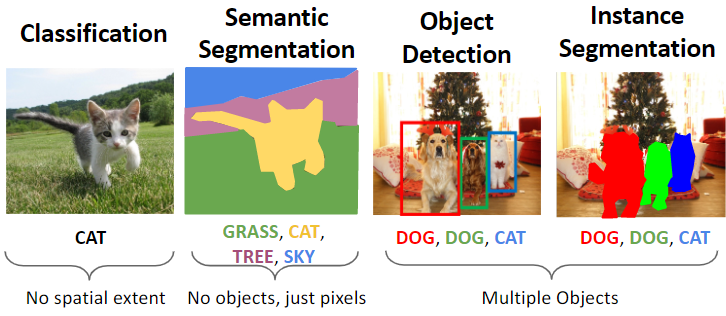
\includegraphics[width=0.68\textwidth]{Lec10/Recognition}
    \caption{Recognition}
\end{figure}


\section{Semantic segmentation(语义分割)}
Input: image

Output: Label each pixel in the image with a category label. Do not differentiate instances. 

\subsection{Sliding window(移动窗口)}
Very inefficient and Limited receptive fields. 效率低下且只有局部信息.  

\begin{figure}[H]
    \centering
    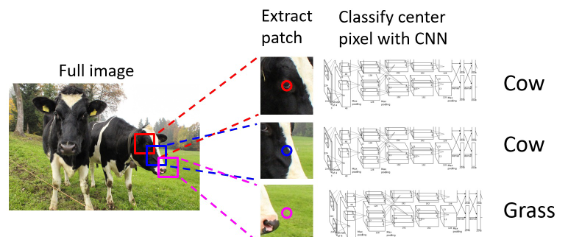
\includegraphics[width=0.48\textwidth]{Lec10/Sliding window}
    \caption{Sliding window}
\end{figure}

\subsection{Fully convolutional network(FCC)}
都是卷积的网络. 从图像到图像, 一次进行整张图的估计, Loss function 就是每个像素的交叉熵(cross-entropy)之和. 

tag是手工标的, 正所谓``多少人工就有多少智能''x

缺点: 可视域仅与层数成线性关系, 且高分辨率下消耗昂贵. 

\begin{figure}[H]
    \centering
    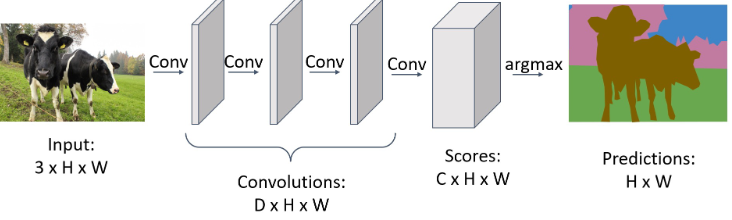
\includegraphics[width=0.68\textwidth]{Lec10/Fully convolutional network}
    \caption{Fully convolutional network}
\end{figure}

To improve efficiency and receptive field: 
\begin{itemize}
    \item Downsampling: pooling, strided conv
    \item Unpooling
\end{itemize}

\begin{figure}[H]
    \centering
    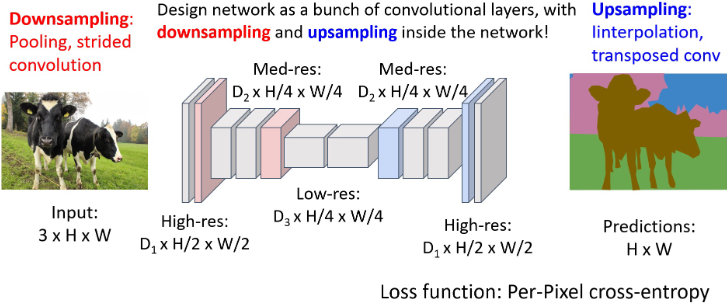
\includegraphics[width=0.68\textwidth]{Lec10/improvement}
    \caption{improvement}
\end{figure}

\subsubsection{Unpooling}
\begin{itemize}
    \item Bed of Nails (填零)
    \item Nearest Neighbor (填周围的)
    \begin{itemize}
        \item Bilinear Interpolation (双线性)
        \item Bicubic Interpolation (双三次)
    \end{itemize}
    \item Transposed convolution (让网络去学习插值)
\end{itemize}

\subsection{U-Net}
Skip connection between downsampling and upsampling stages. (使用跳过层来保留信息) 也叫 hourglass-net

\begin{figure}[H]
    \centering
    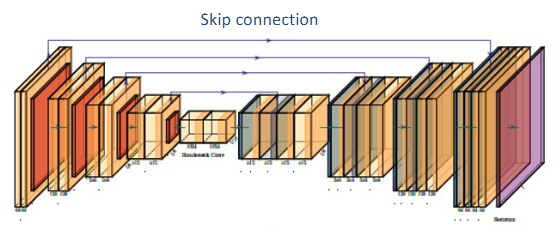
\includegraphics[width=0.68\textwidth]{Lec10/U-Net}
    \caption{U-Net}
\end{figure}

\subsection{DeepLab}
FCN + CRF, 现阶段最好的方式

DCNN(膨胀卷积): 间隔卷积, 让卷积核更大但算量减少? 

\begin{figure}[H]
    \centering
    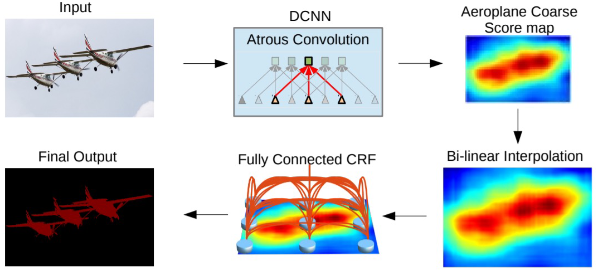
\includegraphics[width=0.68\textwidth]{Lec10/DeepLab}
    \caption{DeepLab}
\end{figure}

\subsubsection{Conditional random field(CRF)}
Energy function: 
\begin{align*}
    E(x)&=\sum_i \theta_i (x_i)+\sum_{ij}\theta_{ij}(x_i,x_j)\\
\end{align*}
\begin{align*}
    \text{Unary potential: }&\, \theta_i (x_i)=-\log P(x_i)\,\,\text{where $P(x_i)$ is the score map given by network}\\
    \text{Pairwise potential: }&\, \theta_{ij}(x_i,x_j)=\mu(x_i,x_j)\left[ w_1 \exp\left(-\frac{\left\| p_i-p_j \right\|^2}{2\sigma_{\alpha}^2}-\frac{\left\| I_i-I_j \right\|^2}{2\sigma_{\beta^2}}\right) + w_2 \exp\left(-\frac{\left\| p_i-p_j \right\|^2}{2\sigma_{\gamma}^2}\right)\right]\\
    & \text{where }\, 
    \mu(x_i,x_j)=\left\{\begin{array}{cc}
        1 & x_i\ne x_j\\
        0 & \text{otherwise}
    \end{array} \right. 
\end{align*}

Pairwise potential: 权重取决于像素是否一致, 若不一致但分数相近也要减小惩罚, 最后捣腾为这个式子. 

\subsection{Evaluation metric(衡量测度)}
Per-pixel Intersection-over-union (IoU), 交集除并集.

mIoU is mean IoU of each categories.

\begin{figure}[H]
    \centering
    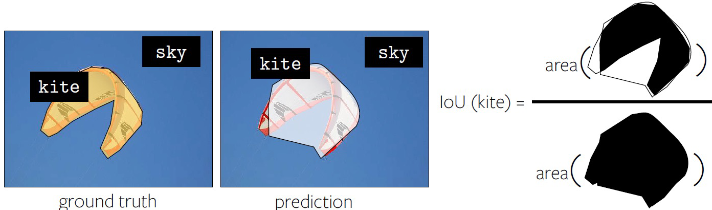
\includegraphics[width=0.68\textwidth]{Lec10/IoU}
    \caption{IoU}
\end{figure}

\section{Object detection}
Input: image

Output: A set of bounding boxes that denote objects. 

Bounding box (bbox):
\begin{itemize}
    \item Class label
    \item Location (x,y)
    \item Size (w,h)
\end{itemize}

\subsection{Detecting a single object}
Treat localization as a regression problem. 

\begin{figure}[H]
    \centering
    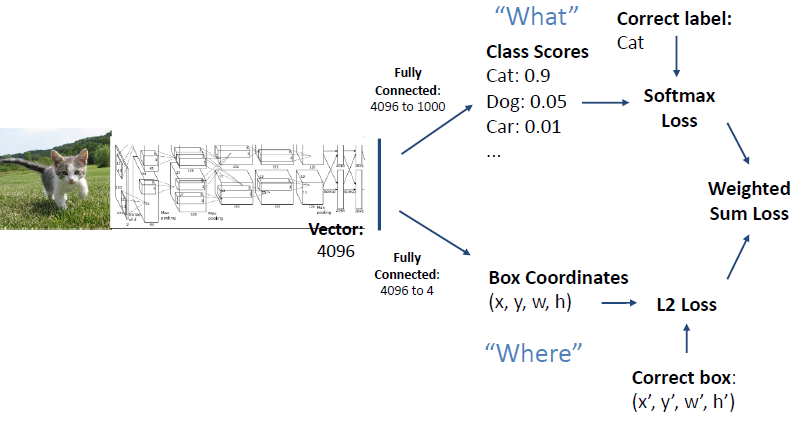
\includegraphics[width=0.68\textwidth]{Lec10/Detecting a single object}
    \caption{Detecting a single object}
\end{figure}

\subsection{Detecting multiple objects}
Bounding box的数量并不一定, 这是最难以解决的地方. 

\subsubsection{Sliding window}
\sout{没错又是我}Apply a CNN to many different crops of the image, CNN classifies each crop as object or background. (直接检测一些框, 名 proposal)

但候选的框太多了, 无法穷举. 

\subsubsection{Region proposals}
Find a small set of boxes that are likely to cover all objects. Often based on heuristics (eg: by over-segmentation). Relatively fast to run.

\begin{figure}[H]
    \centering
    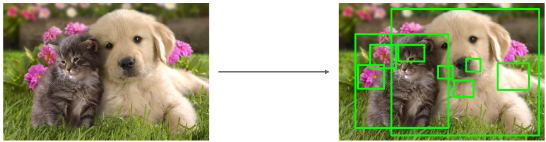
\includegraphics[width=0.68\textwidth]{Lec10/Region proposals}
    \caption{Region proposals}
\end{figure}

\subsubsection{R-CNN}
\begin{enumerate}
    \item Run region proposal method to compute ~2000 region proposals. 
    \item Resize each region to 224x224 and run through CNN. 
    \item Predict class scores and bbox transform.
    \item Use scores to select a subset of region proposals to output. 
\end{enumerate}

\begin{figure}[H]
    \centering
    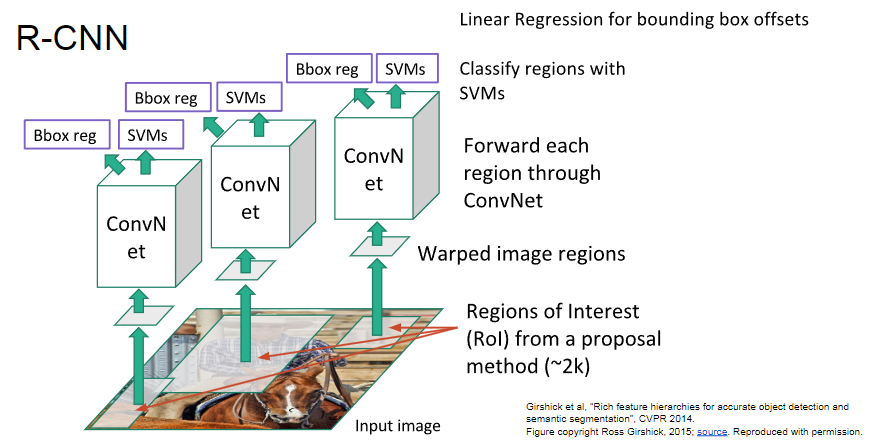
\includegraphics[width=0.48\textwidth]{Lec10/R-CNN}
    \caption{R-CNN}
\end{figure}

\subsection{Evaluation metric}

\subsubsection{For detecting a single object}
\begin{align*}
    \text{Intersection over Union (IoU) }= \frac{\text{Area of Intersection}}{\text{Area of Union}}
\end{align*}

\begin{itemize}
    \item IoU>0.5 is decent. 
    \item IoU>0.7 is pretty good. 
    \item IoU>0.9 is almost perfect. 
\end{itemize}

\subsubsection{For Detecting multiple objects}

\begin{itemize}
    \item Positives and negatives:
    \begin{itemize}
        \item True positive (TP)
        \item False positive (FP)
        \item True negative (TN)
        \item False negative (FN)
    \end{itemize}
    \item Precision(精度) = TP/(TP+FP) 
    \item Recall(召回率) = TP/(TP+FN)
\end{itemize}

\begin{figure}[H]
    \centering
    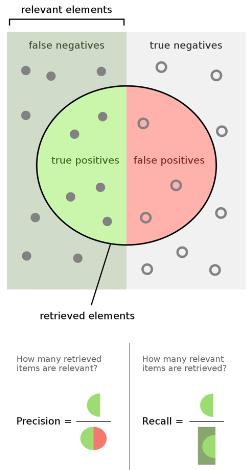
\includegraphics[width=0.3\textwidth]{Lec10/Evaluation metric for Detecting multiple objects}
    \caption{Precision and recall}
\end{figure}

\subsubsection{Mean Average Precision (mAP)}
\begin{multicols}{2}
    
    \begin{enumerate}
        \item Run object detector on all test images.
        \item For each category, compute Average Precision(AP) = area under Precision vs Recall Curve.
        \begin{enumerate}
            \item For each detection (highest score to lowest score).
            \begin{enumerate}
                \item If it matches some ground-truth box with IoU > 0.5, mark it as positive and eliminate the ground-truth.
                \item Otherwise mark it as negative.
                \item Plot a point on PR Curve. 
            \end{enumerate}
            \item Average Precision (AP) = area under PR curve.
            \item Mean Average Precision (mAP) = average of AP for each category. 
            \item For “COCO mAP”: Compute mAP for each IoU threshold(阈值) (0.5, 0.55, 0.6, ..., 0.95) and take average. 
        \end{enumerate}
    \end{enumerate}

    \columnbreak
    
    \begin{figure}[H]
        \centering
        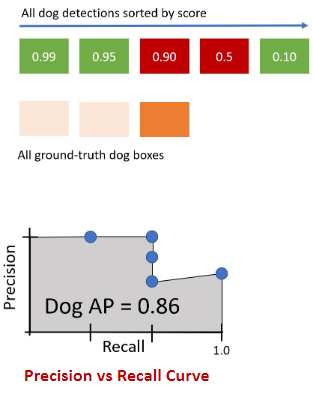
\includegraphics[width=0.28\textwidth]{Lec10/Mean Average Precision}
        \caption{Mean Average Precision}
    \end{figure}

\end{multicols}
To get AP = 1.0: 
Hit all GT boxes with IoU > 0.5, and have no ``false positive'' detections ranked above any ''true positives''.

\subsubsection{Non-Max Suppression(非极大值抑制)}

Object detectors often output many overlapping detections. (把和最大分数重合超过阈值的框去了) 

\begin{wrapfigure}[10]{r}{0.48\textwidth}
    \centering
    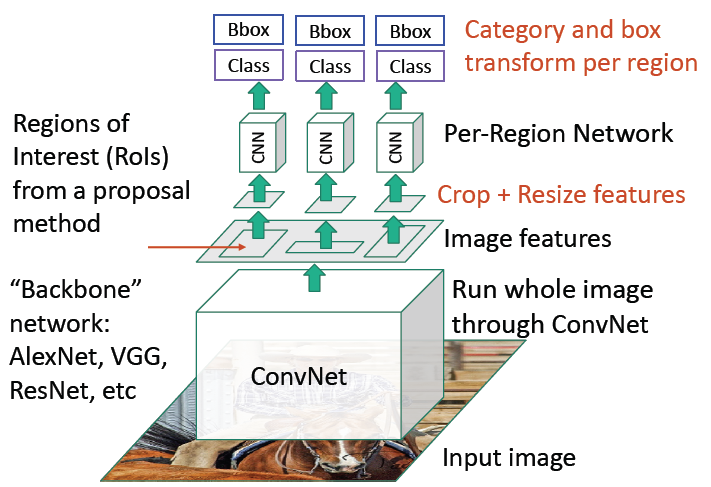
\includegraphics[width=0.48\textwidth]{Lec10/Fast R-CNN}
    \caption{Fast R-CNN}
\end{wrapfigure}

\quad

\begin{enumerate}
    \item Select the highest-scoring box.
    \item Eliminate lower-scoring boxes with IoU > threshold.
    \item If any boxes remain, goto 1. 
\end{enumerate}

\subsection{Fast R-CNN}

R-CNN不够快(本质是每个框单独过网络), 就有了Fast R-CNN.

\begin{enumerate}
    \item ``Backbone''(骨干网络): 特征提取, 先整张图过一次网络得特征图, 以此再用proposal过可以减少每次的网络深度.
    \item Regions of Interest (RoIs) pooling: 将不同的proposal同化
\end{enumerate}

\subsection{Faster R-CNN/Two-stage}
Use CNN to select proposals, called Region Proposal Network (RPN). (加速了proposal生成的部分)

\begin{enumerate}
    \item Run once per image
    \begin{enumerate}
        \item Backbone network
        \item RPN
    \end{enumerate}
    \item Run once per region
    \begin{enumerate}
        \item Crop features Rol pool/align
        \item Predict object class
        \item Predict bbox offset
    \end{enumerate}
\end{enumerate}

\begin{figure}[H]
    \centering
    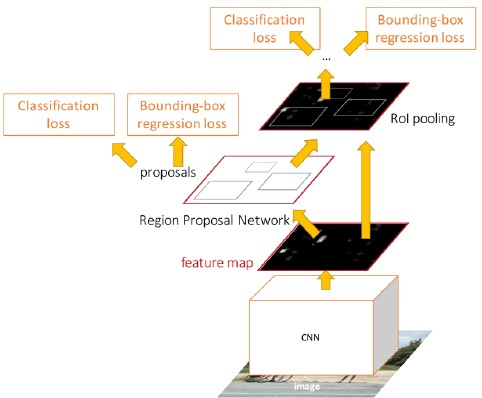
\includegraphics[width=0.28\textwidth]{Lec10/Faster R-CNN}
    \caption{Faster R-CNN}
\end{figure}

\subsubsection{RPN}
Imagine an anchor box(算是候选的bbox) of fixed size at each point in the feature map. 

先生成k个框(预先给予了), 再过网络判断k个框的好坏(RPN). 过网络同时也调整了最好的box. 

\begin{figure}[H]
    \centering
    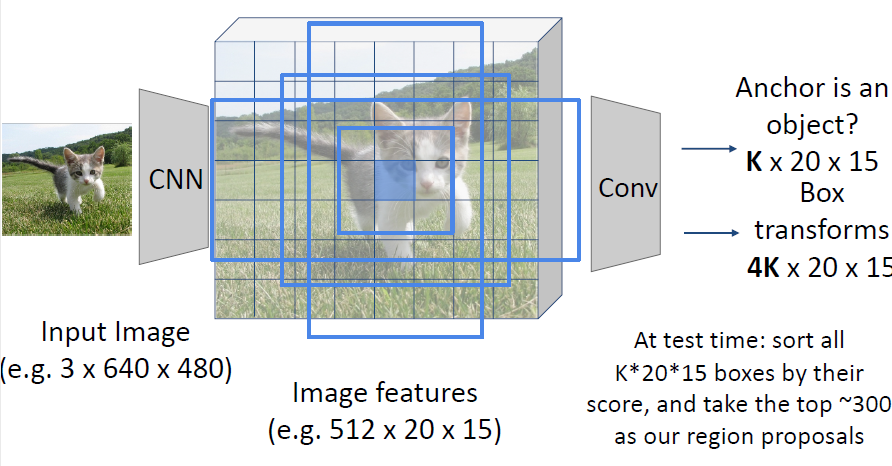
\includegraphics[width=0.68\textwidth]{Lec10/RPN}
    \caption{RPN}
\end{figure}

\subsection{Single-stage object detection}
RPN: Classify each anchor as object / not object.

Single-Stage Detector: Classify each object as one of C categories (or background).

(相当于直接在分类时判断类别)

\subsubsection{YOLO detector}
原作者只到了v4
\begin{figure}[H]
    \centering
    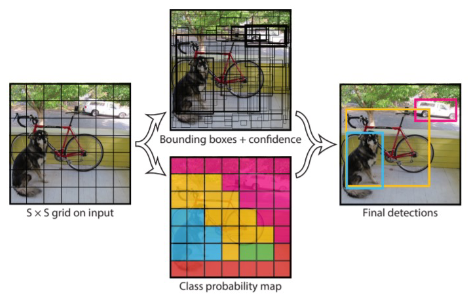
\includegraphics[width=0.48\textwidth]{Lec10/YOLO}
    \caption{YOLO}
\end{figure}

\subsection{Two-stage or Single-stage}
Two-stage is generally more accurate. Single-stage is faster. 

\section{Instance segmentation(实例分割)}
Detect all objects in the image, and identify the pixels that belong to each object (Only things). Perform object detection, then predict a segmentation mask for each object.

\subsection{Mask R-CNN}
Faster R-CNN + additional head

\begin{figure}[H]
    \centering
    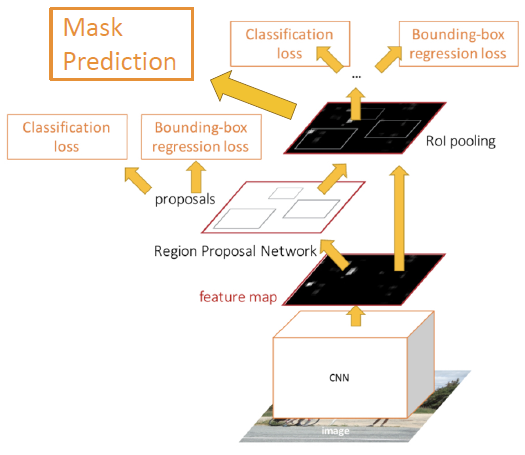
\includegraphics[width=0.38\textwidth]{Lec10/Mask R-CNN}
    \caption{Mask R-CNN}
\end{figure}

\subsection{Deep snake}
传统的算法. 训网络调整框. 

\begin{figure}[H]
    \centering
    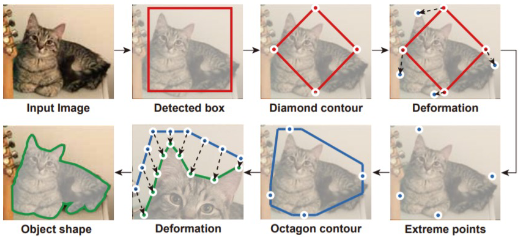
\includegraphics[width=0.618\textwidth]{Lec10/Deep snake}
    \caption{Deep snake}
\end{figure}

\subsection{Panoptic segmentation(全景分割)}
语义+实例 (背景也要分类)

\begin{figure}[H]
    \centering
    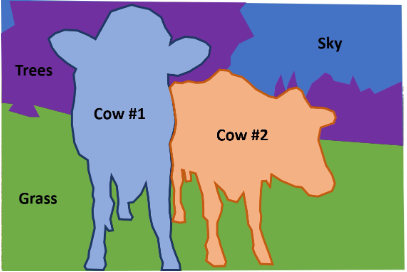
\includegraphics[width=0.38\textwidth]{Lec10/Panoptic segmentation}
    \caption{Panoptic segmentation}
\end{figure}


\subsection{Datasets}
Microsoft COCO (现在最常用的数据集)
\begin{itemize}
    \item 118K train
    \item 5K val
    \item Contains
    \begin{itemize}
        \item Object detection
        \item Keypoints
        \item Instance seg
        \item Panoptic seg
    \end{itemize}
\end{itemize}

\section{Human pose estimation}

\subsection{Represent the pose of a human}

\begin{wrapfigure}[8]{r}{0.38\textwidth}
    \centering
    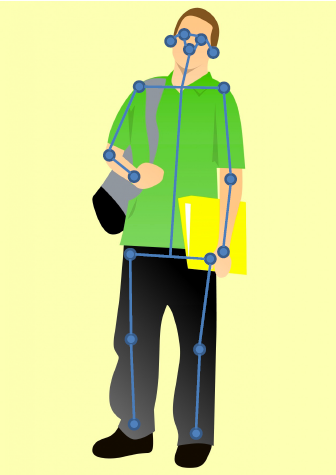
\includegraphics[width=0.38\textwidth]{Lec10/Represent the pose of a human}
    \caption{Represent the pose of a human}
\end{wrapfigure}


Represent the pose of a human by locating a set of keypoints.

e.g. 17 keypoints:
\begin{itemize}
    \item Nose
    \item Left / Right eye
    \item Left / Right ear
    \item Left / Right shoulder
    \item Left / Right elbow
    \item Left / Right wrist
    \item Left / Right hip
    \item Left / Right knee
    \item Left / Right ankle
\end{itemize}

\subsection{Human pose estimation with depth sensors}
Microsfot Kinect, 基于深度相机识别人体关键部位. 

\subsection{Single human}

\subsubsection{Directly predict}
Directly predict joint locations (a 17*2 vector). 

图转向量需要很多全连接层, 难以训练, 图像到坐标的映射也难以学习. 

\subsubsection{heatmap}
Represent joint location as the heatmap(热力图).

一个heatmap代表一个关键点. 输出变成图了, 只需要卷积了. 

\begin{figure}[H]
    \centering
    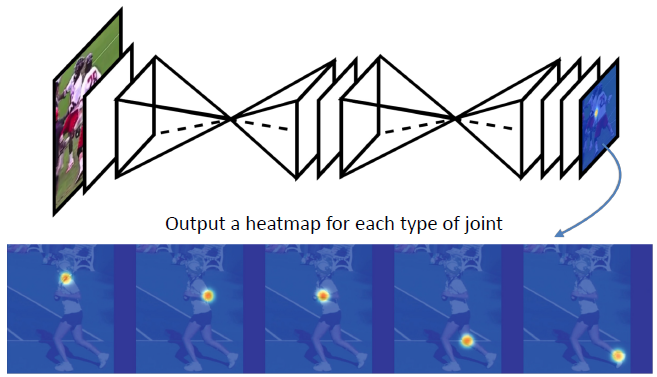
\includegraphics[width=0.618\textwidth]{Lec10/heatmap}
    \caption{heatmap}
\end{figure}

\begin{wrapfigure}[7]{r}{0.38\textwidth}
    \centering
    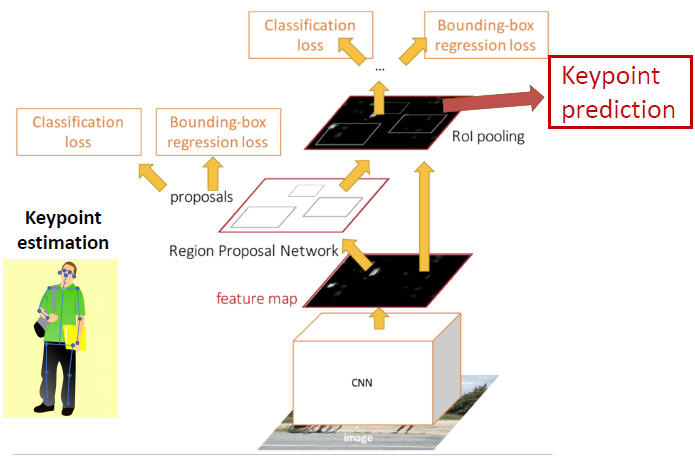
\includegraphics[width=0.38\textwidth]{Lec10/Mask R-CNN-pose}
    \caption{Mask R-CNN-pose}
\end{wrapfigure}

\quad

\subsection{Multiple humans}

\subsubsection{Top-down}

Detect humans and detect keypoints in each bbox. Example: Mask R-CNN. 最大问题还是慢了. 

% \begin{figure}[H]
%     \centering
%     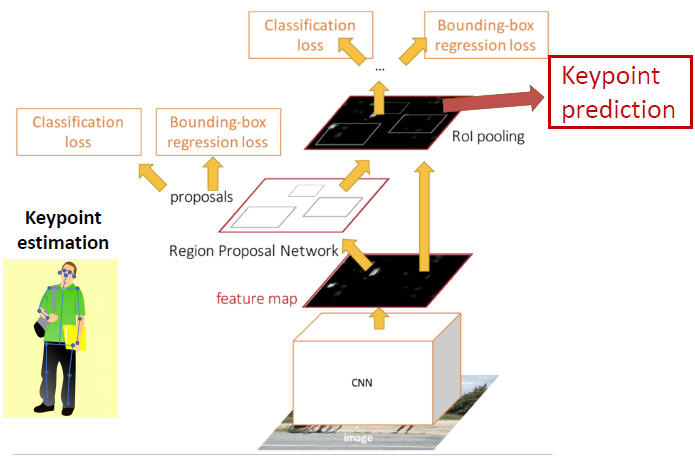
\includegraphics[width=0.38\textwidth]{Lec10/Mask R-CNN-pose}
%     \caption{Mask R-CNN-pose}
% \end{figure}


\subsubsection{Bottom-up}
Detect keypoints and group keypoints to form humans.Example: OpenPose. 

\begin{enumerate}
    \item Part affinity fields. 
    \begin{figure}[H]
        \centering
        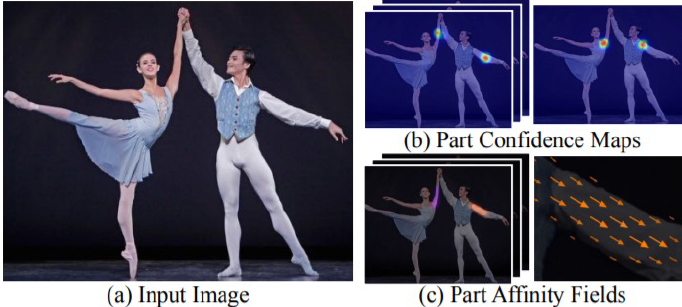
\includegraphics[width=0.618\textwidth]{Lec10/Part affinity fields}
        \caption{Part affinity fields}
    \end{figure}
    
    \item Link parts based on part affinity fields. 
    
    \begin{figure}[H]
        \centering
        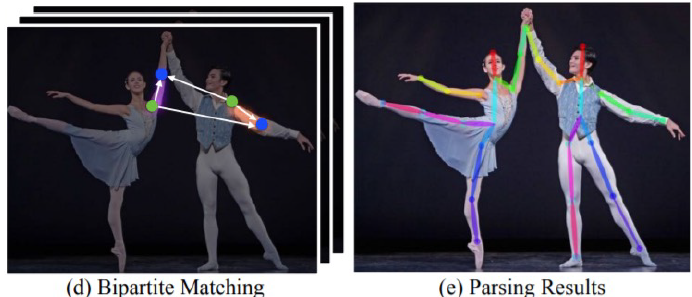
\includegraphics[width=0.618\textwidth]{Lec10/Link parts}
        \caption{Link parts}
    \end{figure}
\end{enumerate}

\subsection{Top-down or bottom-up}
Top-down is generally more accurate. Bottom-up is faster. (Bottom-up 在有遮挡下也有优势)

\section{Other tasks}

\subsection{Video classification}

\begin{figure}[H]
    \centering
    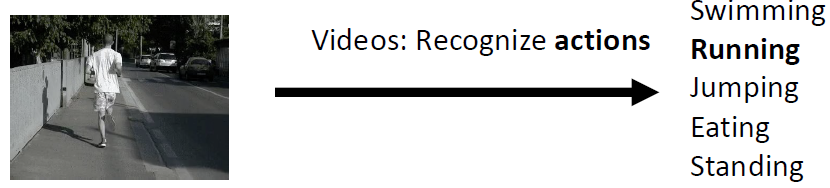
\includegraphics[width=0.518\textwidth]{Lec10/Video classification}
    \caption{Video classification}
\end{figure}

Use 3D CNN. (时间也是个维度)

\begin{figure}[H]
    \centering
    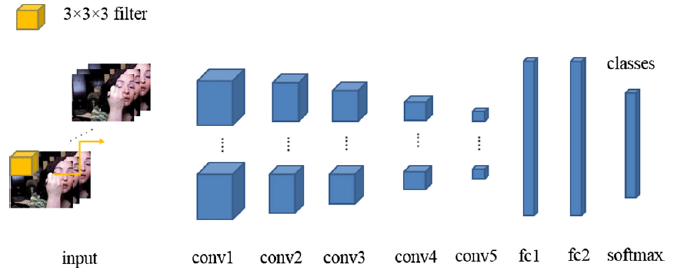
\includegraphics[width=0.518\textwidth]{Lec10/3D CNN}
    \caption{3D CNN}
\end{figure}

\subsection{Temporal action localization}
Given a long untrimmed video sequence, identify frames corresponding to different actions. Generate proposals then classify. 

\begin{figure}[H]
    \centering
    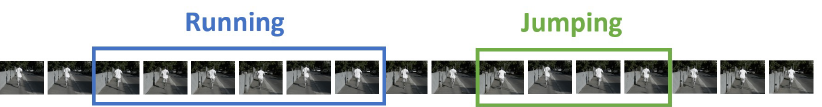
\includegraphics[width=0.518\textwidth]{Lec10/Temporal action localization}
    \caption{Temporal action localization}
\end{figure}

\subsection{Spatial-temporal detection}
Given a long untrimmed video, detect all the people in space and time and classify the activities they are performing. 

\begin{figure}[H]
    \centering
    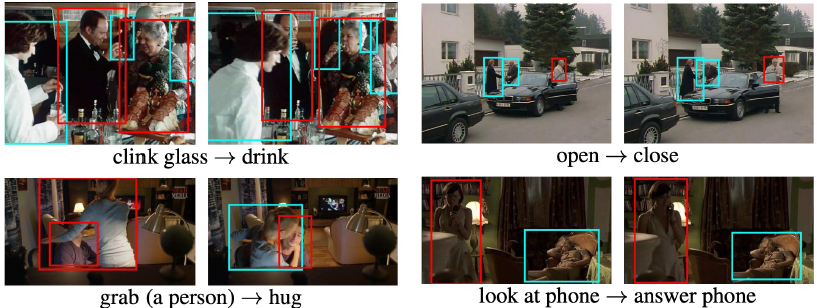
\includegraphics[width=0.518\textwidth]{Lec10/Spatial-temporal detection}
    \caption{Spatial-temporal detection}
\end{figure}

\subsection{Multi-object tracking}
Identify and track objects belonging to one or more categories without any prior knowledge about the appearance and number of targets.

\subsection{Papers with code}

\href{https://paperswithcode.com/sota}{paperswithcode.com}

去看本领域较优的方法, 可以参考(它只是个非专业网站, 排名有局限性, 不可全信), 需要进一步的挖掘的. 